\chapter{Mô hình giải pháp}

\section{Mô hình tổng thể}

Mô hình tổng thể cho kho dữ liệu ebook online sẽ bao gồm 4 thành phần chính:

\begin{equation}
    \text{(D, FS, DB, ONT)}
\end{equation}

Trong đó:

\begin{itemize}
    \item \textit{D (Document)} là tập các tài liệu được quản lý trong hệ thống. Bên cạnh nội dung của mình, mỗi tài liệu có một định danh riêng biệt, có các thông tin siêu dữ liệu liên quan và ngữ nghĩa của tài liệu được biểu diễn bằng một đô thị key phrase. 
    \item \textit{FS (File system)} là hệ thống tập tin dùng để lưu trữ các chế bản điện tử của
tài liệu trong hệ thống. Đây là thành phần cơ bản của một kho tài liệu điện tử và là cấp thấp nhất về mặt lưu trữ trong hệ thống.

    \item \textit{DB (Database)} Cơ sở dữ liệu danh mục. Database lưu trữ thông tin siêu dữ liệu liên quan đến tài liệu cùng cấu trúc thư mục của hệ thống tập tin (File system). Đóng vai trò liên kết giữa File system với các thành phần trừu tượng khác trong hệ thống.
    
    \item \textit{ONT (Ontology)} là mô hình ontology cho ngữ nghĩa của tài liệu, chi phối quá
trình các thao tác xử lý liên quan đến ngữ nghĩa của tài liệu.
\end{itemize}



\section{Mô hình Ontology biểu diễn ngữ nghĩa: CK-ONT}

Mô hình được đề xuất để biểu diễn hệ thống tìm kiếm theo ngữ nghĩa dựa trên ontology là mô hình CK-ONT (Classed Keyphrase based Ontology). Mô hình gồm 6 thành phần. 

\begin{equation}
    \centering
    (K, C, R_{KC}, R_{CC}, R_{KK}, label)
\end{equation}

Trong phạm vi nghiên cứu, mô hình CK-OB được kế thừa từ mô hình CK-ONT và đưa vào sử dụng dùng để mô hình hóa cho các tài liệu là ebook lĩnh vực CNTT, mô hình gồm 5 thành phần như sau: 

\begin{equation}
    \centering
    (K, C, R_{KC}, R_{CC}, R_{KK})
\end{equation}

Trong đó:
\begin{itemize}
    \item K: tập hợp các Keyphrase thuộc lĩnh vực CNTT.
    \item C: tập hợp các lớp keyphrase
    \item $R_{KC}$: tập hợp các quan hệ giữa keyphrase và lớp.
    \item $R_{CC}$: tập hợp các quan hệ giữa các lớp.
    \item $R_{KK}$: tập hợp quan hệ giữa các keyphrase.
\end{itemize}

\subsection{Tập hợp K các keyphrase}

\begin{itemize}
    \item Là thành phần chính hình thành nên các khái niệm của ontology.
    \item Keyphrase trong mô hình này là những cụm từ hay thuật ngữ chuyên ngành CNTT. \\
    Ví dụ: "lập trình", "con trỏ", "bool", ...
\end{itemize}

\subsection{Tập hợp C các lớp keyphrase}

\begin{itemize}
    \item Môi lớp keyphrase là một tập hợp các keyphrase có liên quan với nhau theo một tính chất hay ngữ nghĩa nào đó
    \item Một lớp keyphrase có thể chứa các keyphrase hoặc các lớp keyphrase.
    \item Khi một lớp có chứa các lớp khác sẽ tạo thành mối quan hệ phân cấp cha con. \\

$C = \{ c \in P(K)\ |\ \text{c là lớp keyphrase mô tả lĩnh vực đang xét} \}$

Ví dụ: Lớp \textit{XuLyNN} chứa các keyphrase liên quan đến xử lý ngôn ngữ tự nhiên như sau:

$XuLyNN = \{ \text{Tách từ, PosTag, TFIDF, phân lớp, Word2vec} \}$

\end{itemize}

\subsection{Tập hợp $R_{KC}$ các quan hệ giữa keyphrase và lớp}

Một quan hệ hai ngôi giữa K và C ($C \neq \emptyset, K \neq \emptyset$) là một tập con của $K \times C$ và $K_{RC} = \{ r\ |\ r \subseteq K \times C \}$.

Trong phạm vi báo cáo này chỉ xét quan hệ \textit{inClass} ("thuộc về") giữa keyphrase và lớp.

Ví dụ: "Tách từ" inClass $XuLyNN$, "TFIDF" inClass $XuLyNN$, ...

\subsection{Tập hợp $R_{CC}$ các quan hệ giữa các lớp}

Một quan hệ hai ngôi trên tập hợp các lớp keyphrase C ($C \neq \emptyset$) là tập con của $C \times C$ và $R_{CC} = \{ r\ |\ r \subseteq C \times C \}$.

Báo cáo chỉ xét quan hệ trên phân cấp lớp.

Ví dụ: Có sơ đồ phân cấp lớp như sau: 

\begin{figure}[H]
    \centering
    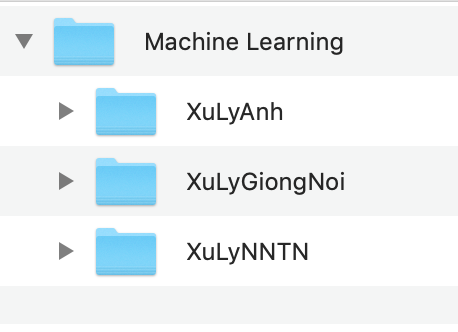
\includegraphics[width=0.5\textwidth]{img/phancapclasses.png}
\end{figure}

trong đó mỗi quan hệ giữa các lớp được mô tả như sau:

\begin{table}[H]
\centering
\begin{tabular}{|l|l|}
\hline
\textbf{SuperClass} & \textbf{SubClass} \\ \hline
Machine Learning    & XuLyAnh           \\ \hline
Machine Learning    & XuLyGiongNoi      \\ \hline
Machine Learning    & XuLyNNTN          \\ \hline
\end{tabular}
\end{table}

\subsection{Tập hợp $R_{KK}$ các quan hệ giữa các keyphrase}
Một quan hệ hai ngôi trên K ($K \neq \emptyset $) là một tập hợp con của $K \times K$ nghĩa là một tập các cặp keyphrase thuộc K và $R_{RR} = \{ r\ |\ r \subseteq K \times K \}$

Trong phạm vi đề tài ta chỉ xét các loại quan hệ sau:

\begin{table}[H]
\centering
\begin{tabular}{|l|l|l|}
\hline
\textbf{} & \textbf{Quan hệ ngữ nghĩa} & \textbf{Mô tả}           \\ \hline
r1        & Đồng nghĩa                 & A đồng nghĩa với B       \\ \hline
r2        & Viết tắt                   & A là dạng viết tắt của B \\ \hline
r3        & Cùng lớp                   & A cùng lớp với B         \\ \hline
\end{tabular}
\end{table}

\begin{itemize}
    \item \textbf{Quan hệ đồng nghĩa r1}: hai keyphrase có quan hệ \textit{đồng nghĩa} nếu chúng cùng nghĩa và thay thế được cho nhau trong một ngữ cảnh nào đó. \\ 
    Ví dụ: keyphrase "công nghệ phần mềm" có quan hệ \textit{đồng nghĩa} với keyphrase "kỹ thuật phần mềm"
    \item \textbf{Quan hệ Viết tắt r2}: hai keyphrase có quan hệ \textit{viết tắt} nếu chúng cùng nghĩa với nhau và thay thế được cho nhau trong một ngữ cảnh nào đó. \\
    Ví dụ: keyphrase "CSS" 
    \item \textbf{Quan hệ Cùng lớp r3}: keyphrase a có quan hệ \textit{cùng lớp} với keyphrase b nếu có một lớp $C_{i}$ sau cho $a \in C_{i}$ và $b \in C_{i}$. \\
    Ví dụ: keyphrase \textit{"Javascript"} có quan hệ cùng lớp với keyphrase \textit{"Typescript"}.
\end{itemize}

\section{Tìm kiếm theo ngữ nghĩa}

\subsection{Công cụ xây dựng Ontology}

Protégé là công cụ phần mềm biên tập ontology mã nguồn mở (được phát triển tại Trường ĐH Stanford) sử dụng đối với việc xây dựng các hệ thống thông minh. Protégé được hỗ trợ bởi cộng đồng lớn bao gồm: các viện nghiên cứu, các tổ chức chính phủ và những người sử dụng cộng tác. Các đơn vị, cá nhân này sử dụng Protégé để xây dựng các giải pháp dựa trên tri thức trong các lĩnh vực chuyên sâu như là: y sinh học, thương mại điện tử và mô hình hóa tổ chức.

Chuẩn ngôn ngữ được sử dụng nhiều nhất để xây dựng ontology hiện nay là OWL\cite{antoniou2004web} được phát triển bởi W3C. Giống như Protégé, OWL có thể mô tả các khái niệm nhưng nó cũng đưa ra các cách thức mới. Nó bao gồm tập rất nhiều các phép toán, ví dụ: phép giao (intersection), phép hợp (union) và phép phủ định (negation). Nó dựa trên một mô hình lo-gic khác giúp nó có thể định nghĩa các khái niệm giống như cách mà các khái niệm đó đã được mô tả.

\subsection{Công cụ lập chỉ mục và tìm kiếm - Apache Solr}

Apache Solr là một nền tảng full-text search mã nguồn mở dựa trên Apache Lucence. Lucene là một thư viện được viết bằng Java dùng để phân tích, đánh chỉ mục (indexing) và tìm kiếm thông tin được phát triển đầu tiên bởi Doug Cutting vào năm 2000. Cutting đồng thời cũng là tác giả của Hadoop lúc ông đang làm việc cho Yahoo vào năm 2005. Solr không hoàn toàn là một RESTful interface của Lucene mà là sử dụng Lucene như là một component trong toàn bộ hệ thống.

Apache Solr có nhiều thành phần chính, nhưng quan trọng nhất là 2 thành phần: Thành phần tạo chỉ mục và thành phần tìm kiếm.


\begin{figure}[H]
    \centering
    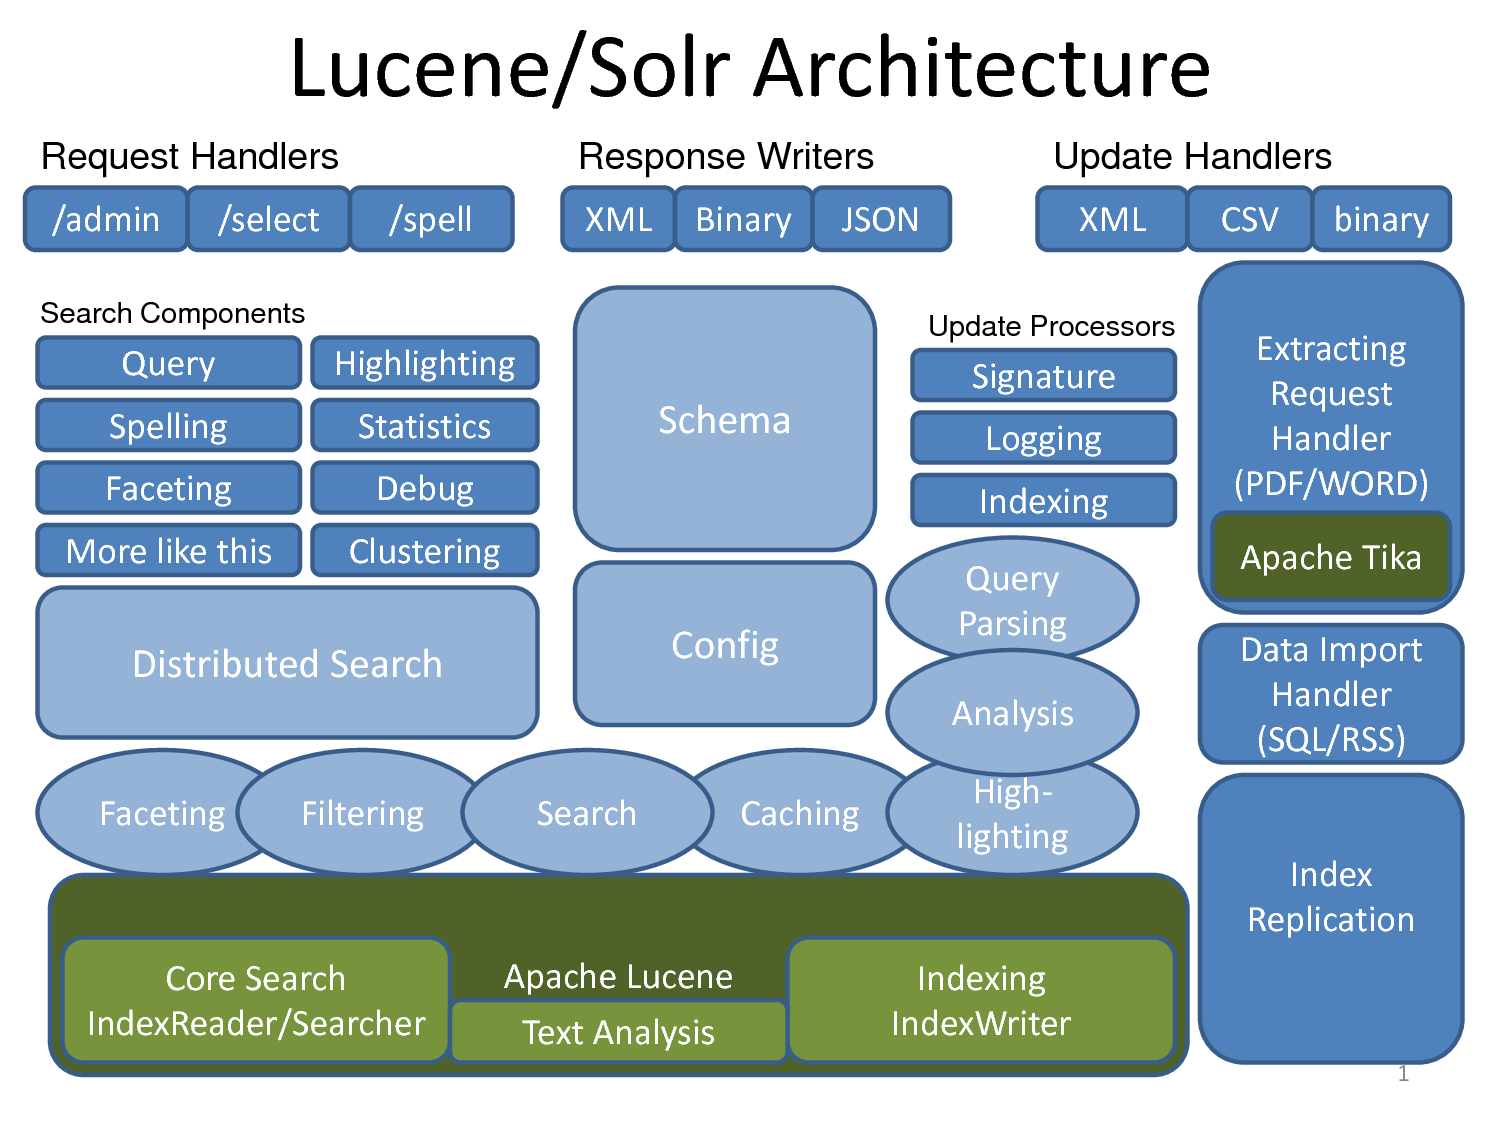
\includegraphics[width=0.8\textwidth]{img/solr-achitecture.png}
    \caption{Các thành phần của Apache Solr}
\end{figure}

\begin{itemize}
    \item \textbf{Thành phần Tạo chỉ mục}: bao gồm các thành phần hỗ trợ xử lý, tạo chỉ mục từ văn bản tài liệu đầu vào và cho ra kết quả là tập chỉ mục phục vụ cho thành phần tìm kiếm. Các component cơ bản bao gồm:
    \begin{itemize}
        \item \textit{Directory}: định nghĩa vùng nhớ, RAM nơi lưu chỉ mục.
        \item \textit{Document và Field}: định nghĩa tài liệu và các trường thông tin của tài liệu cho việc lập chỉ mục, dùng cho việc trả kết quả cho tìm kiếm.
        \item\textit{Analyzer}: thực hiện chức năng xử lý và tách văn bản để lấy nội dung, chuẩn hóa, loại bỏ từ không cần thiết, ... hỗ trợ cho bước lập chỉ mục. \\
        Analyzer đóng vai trò khảo sát các trường văn bản để tạo ra một token stream. Ví dụ: \textit{WhitespaceAnalyzer} xử lý phân tích văn bản thành những token dựa trên khoảng trắng. Câu \textit{"The quick brown fox jump over the lazy dog"} sẽ được phân tích thành các tokens: \textit{[The] [quick] [brown] [fox] [jump] [over] [the] [lazy] [dog]}.
        
        \item\textit{Tokenizer} Nếu như Analyzer tạo ra các token streams/input stream, thì Tokenizer chia nhỏ các stream đó thành những tokens (đơn vị nhỏ nhất để index, có thể là từ hay ký tự). Các ký tự trong input stream có thể bị bỏ qua như các ký tự không nhìn thấy được (whitespace như khoảng trắng, tab) hay các dấu phân cách (delimiter như dấu phẩy, dấu chấm).

        \item\textit{IndexWriter} thực hiện việc tạo mới, mở chỉ mục, thêm hoặc cập nhật nội dung chỉ mục. Đầy là thành phần chính trong thành phần tạo chỉ mục.
    \end{itemize}
    
    \item\textbf{Thành phần Tìm kiếm} bao gồm các thành phần chức năng phục vụ cho việc xử lý tìm kiếm từ yêu cầu người dùng. Solr hỗ trợ nhiều loại truy vấn khác nhau, cho phép tìm theo trường thông tin hay các thiết lập nâng cao như sắp xếp kết quả, giới hạn thời gian hoặc số lượng kết quả, ... \\
    Các chức năng cơ bản gồm:
    \begin{itemize}
        \item\textit{Term}: là đơn vị cơ bản của tìm kiếm, gồm tên và giá trị tương ứng.
        \item\textit{Query} gồm nhiều loại truy vấn, chứa nhiều phương thức, thiết lập chỉ số Boost nhằm giúp xác định truy vấn con nào quan trọng hơn.
        \item\textit{IndexSearcher} tìm kiếm trên tập chỉ mục \textit{IndexWriter} tạo ra.
    \end{itemize}
\end{itemize}

\subsection{Quá trình thiết lập}

\begin{itemize}
    \item Xây dựng tập chỉ mục tìm kiếm
    \begin{itemize}
        \item Mô hình hóa nội dung với Apache Solr
        \item Tiến trình lập chỉ mục
    \end{itemize}
    
    \item Tìm kiếm trên tập chỉ mục
\end{itemize}
